\documentclass{standalone}
\usepackage{tikz}
\usetikzlibrary{patterns, positioning}


\begin{document}
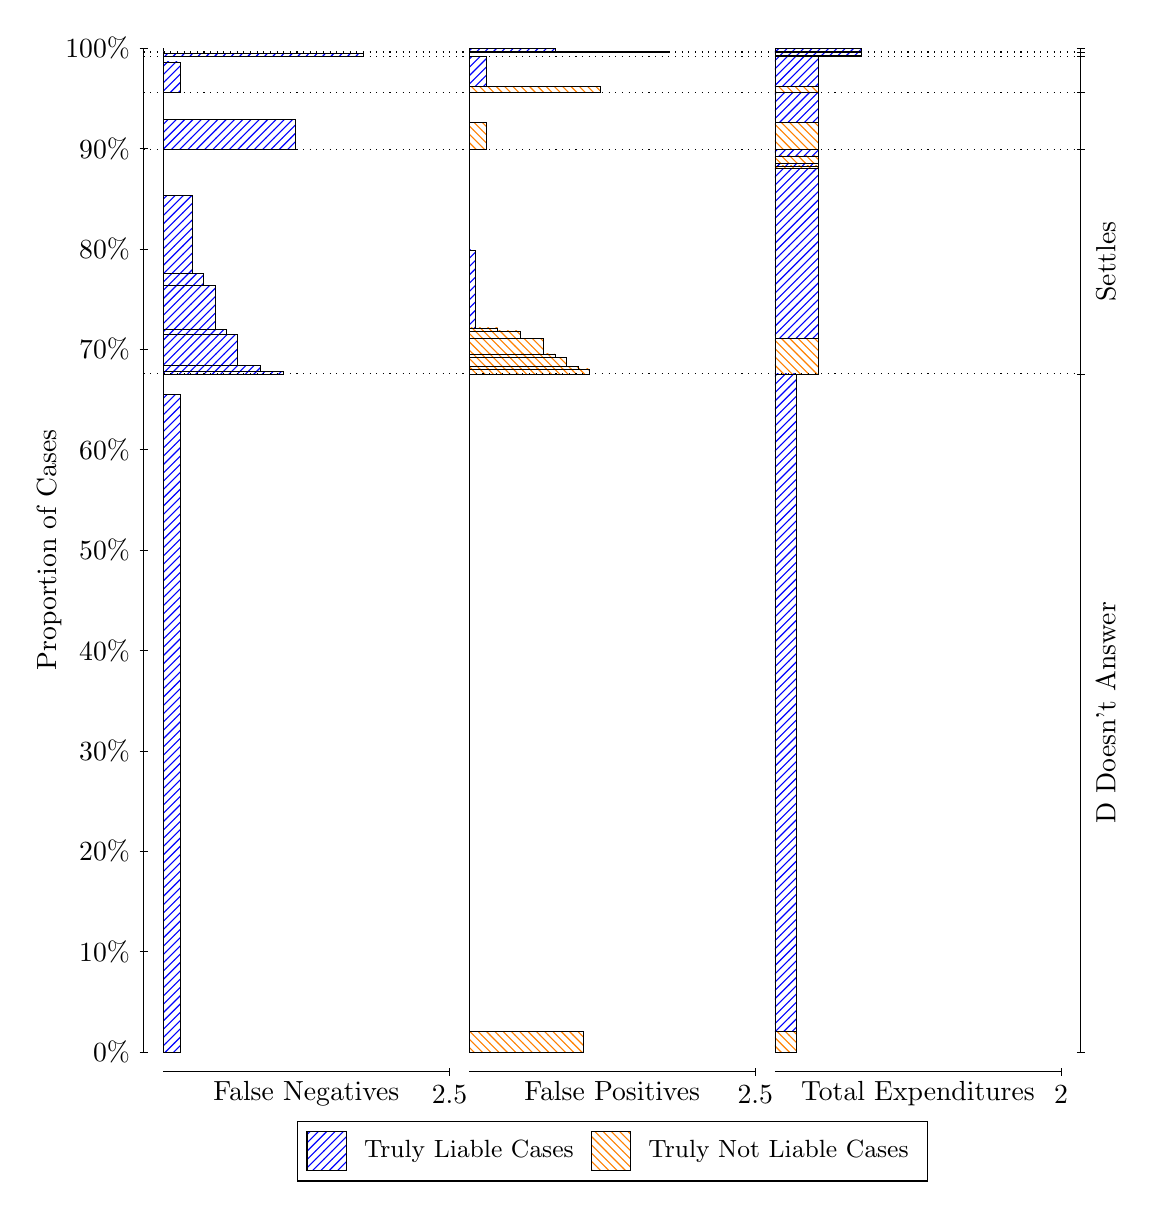
\begin{tikzpicture}
\draw[black, very thin] (1.5,1.75) -- (1.5,14.5);
\node[rotate=90, text=black, anchor=center] at (0.3, 8.125) {Proportion of Cases};
\draw[black, very thin] (1.45,1.75) -- (1.55,1.75);
\node[text=black, anchor=east] at (1.45, 1.75) {0\%};
\draw[black, very thin] (1.45,3.025) -- (1.55,3.025);
\node[text=black, anchor=east] at (1.45, 3.025) {10\%};
\draw[black, very thin] (1.45,4.3) -- (1.55,4.3);
\node[text=black, anchor=east] at (1.45, 4.3) {20\%};
\draw[black, very thin] (1.45,5.575) -- (1.55,5.575);
\node[text=black, anchor=east] at (1.45, 5.575) {30\%};
\draw[black, very thin] (1.45,6.85) -- (1.55,6.85);
\node[text=black, anchor=east] at (1.45, 6.85) {40\%};
\draw[black, very thin] (1.45,8.125) -- (1.55,8.125);
\node[text=black, anchor=east] at (1.45, 8.125) {50\%};
\draw[black, very thin] (1.45,9.4) -- (1.55,9.4);
\node[text=black, anchor=east] at (1.45, 9.4) {60\%};
\draw[black, very thin] (1.45,10.675) -- (1.55,10.675);
\node[text=black, anchor=east] at (1.45, 10.675) {70\%};
\draw[black, very thin] (1.45,11.95) -- (1.55,11.95);
\node[text=black, anchor=east] at (1.45, 11.95) {80\%};
\draw[black, very thin] (1.45,13.225) -- (1.55,13.225);
\node[text=black, anchor=east] at (1.45, 13.225) {90\%};
\draw[black, very thin] (1.45,14.5) -- (1.55,14.5);
\node[text=black, anchor=east] at (1.45, 14.5) {100\%};

\draw[black, very thin] (13.4,1.75) -- (13.4,14.5);
\draw[black, very thin] (13.35,1.75) -- (13.45,1.75);
\node[anchor=west] at (13.35, 1.75) {};
\draw[black, very thin] (13.35,10.362) -- (13.45,10.362);
\node[anchor=west] at (13.35, 10.362) {};
\draw[black, very thin] (13.35,13.213) -- (13.45,13.213);
\node[anchor=west] at (13.35, 13.213) {};
\draw[black, very thin] (13.35,13.936) -- (13.45,13.936);
\node[anchor=west] at (13.35, 13.936) {};
\draw[black, very thin] (13.35,14.397) -- (13.45,14.397);
\node[anchor=west] at (13.35, 14.397) {};
\draw[black, very thin] (13.35,14.45) -- (13.45,14.45);
\node[anchor=west] at (13.35, 14.45) {};
\draw[black, very thin] (13.35,14.5) -- (13.45,14.5);
\node[anchor=west] at (13.35, 14.5) {};

\draw[black, very thin, pattern color=blue, pattern=north east lines] (1.75,1.75) rectangle (1.968,10.101);
\draw[black, very thin, pattern color=orange, pattern=north west lines] (1.75,10.101) rectangle (1.75,10.362);
\draw[black, very thin, pattern color=blue, pattern=north east lines] (1.75,10.362) rectangle (3.276,10.39);
\draw[black, very thin, pattern color=blue, pattern=north east lines] (1.75,10.39) rectangle (2.9853,10.472);
\draw[black, very thin, pattern color=blue, pattern=north east lines] (1.75,10.472) rectangle (2.84,10.474);
\draw[black, very thin, pattern color=blue, pattern=north east lines] (1.75,10.474) rectangle (2.6947,10.863);
\draw[black, very thin, pattern color=blue, pattern=north east lines] (1.75,10.863) rectangle (2.5493,10.927);
\draw[black, very thin, pattern color=blue, pattern=north east lines] (1.75,10.927) rectangle (2.404,11.481);
\draw[black, very thin, pattern color=blue, pattern=north east lines] (1.75,11.481) rectangle (2.2587,11.638);
\draw[black, very thin, pattern color=blue, pattern=north east lines] (1.75,11.638) rectangle (2.1133,12.63);
\draw[black, very thin, pattern color=orange, pattern=north west lines] (1.75,12.63) rectangle (1.75,13.213);
\draw[black, very thin, pattern color=blue, pattern=north east lines] (1.75,13.213) rectangle (3.4213,13.597);
\draw[black, very thin, pattern color=orange, pattern=north west lines] (1.75,13.597) rectangle (1.75,13.936);
\draw[black, very thin, pattern color=blue, pattern=north east lines] (1.75,13.936) rectangle (1.968,14.323);
\draw[black, very thin, pattern color=orange, pattern=north west lines] (1.75,14.323) rectangle (1.75,14.397);
\draw[black, very thin, pattern color=blue, pattern=north east lines] (1.75,14.397) rectangle (4.2933,14.436);
\draw[black, very thin, pattern color=orange, pattern=north west lines] (1.75,14.436) rectangle (1.75,14.45);
\draw[black, very thin, pattern color=orange, pattern=north west lines] (1.75,14.45) rectangle (1.75,14.454);
\draw[black, very thin, pattern color=blue, pattern=north east lines] (1.75,14.454) rectangle (1.75,14.5);
\draw[black, very thin, pattern color=orange, pattern=north west lines] (5.6333,1.75) rectangle (7.0867,2.0116);
\draw[black, very thin, pattern color=blue, pattern=north east lines] (5.6333,2.0116) rectangle (5.6333,10.362);
\draw[black, very thin, pattern color=orange, pattern=north west lines] (5.6333,10.362) rectangle (7.1593,10.424);
\draw[black, very thin, pattern color=orange, pattern=north west lines] (5.6333,10.424) rectangle (7.014,10.453);
\draw[black, very thin, pattern color=orange, pattern=north west lines] (5.6333,10.453) rectangle (6.8687,10.568);
\draw[black, very thin, pattern color=orange, pattern=north west lines] (5.6333,10.568) rectangle (6.7233,10.615);
\draw[black, very thin, pattern color=orange, pattern=north west lines] (5.6333,10.615) rectangle (6.578,10.811);
\draw[black, very thin, pattern color=orange, pattern=north west lines] (5.6333,10.811) rectangle (6.4327,10.813);
\draw[black, very thin, pattern color=orange, pattern=north west lines] (5.6333,10.813) rectangle (6.2873,10.909);
\draw[black, very thin, pattern color=orange, pattern=north west lines] (5.6333,10.909) rectangle (5.9967,10.946);
\draw[black, very thin, pattern color=blue, pattern=north east lines] (5.6333,10.946) rectangle (5.706,11.937);
\draw[black, very thin, pattern color=blue, pattern=north east lines] (5.6333,11.937) rectangle (5.6333,13.213);
\draw[black, very thin, pattern color=orange, pattern=north west lines] (5.6333,13.213) rectangle (5.8513,13.551);
\draw[black, very thin, pattern color=blue, pattern=north east lines] (5.6333,13.551) rectangle (5.6333,13.936);
\draw[black, very thin, pattern color=orange, pattern=north west lines] (5.6333,13.936) rectangle (7.3047,14.01);
\draw[black, very thin, pattern color=blue, pattern=north east lines] (5.6333,14.01) rectangle (5.8513,14.397);
\draw[black, very thin, pattern color=orange, pattern=north west lines] (5.6333,14.397) rectangle (5.6333,14.411);
\draw[black, very thin, pattern color=blue, pattern=north east lines] (5.6333,14.411) rectangle (5.6333,14.45);
\draw[black, very thin, pattern color=orange, pattern=north west lines] (5.6333,14.45) rectangle (8.1767,14.454);
\draw[black, very thin, pattern color=blue, pattern=north east lines] (5.6333,14.454) rectangle (6.7233,14.5);
\draw[black, very thin, pattern color=orange, pattern=north west lines] (9.5167,1.75) rectangle (9.7892,2.0116);
\draw[black, very thin, pattern color=blue, pattern=north east lines] (9.5167,2.0116) rectangle (9.7892,10.362);
\draw[black, very thin, pattern color=orange, pattern=north west lines] (9.5167,10.362) rectangle (10.062,10.811);
\draw[black, very thin, pattern color=blue, pattern=north east lines] (9.5167,10.811) rectangle (10.062,12.967);
\draw[black, very thin, pattern color=orange, pattern=north west lines] (9.5167,12.967) rectangle (10.062,13.004);
\draw[black, very thin, pattern color=blue, pattern=north east lines] (9.5167,13.004) rectangle (10.062,13.032);
\draw[black, very thin, pattern color=orange, pattern=north west lines] (9.5167,13.032) rectangle (10.062,13.129);
\draw[black, very thin, pattern color=blue, pattern=north east lines] (9.5167,13.129) rectangle (10.062,13.213);
\draw[black, very thin, pattern color=orange, pattern=north west lines] (9.5167,13.213) rectangle (10.062,13.551);
\draw[black, very thin, pattern color=blue, pattern=north east lines] (9.5167,13.551) rectangle (10.062,13.936);
\draw[black, very thin, pattern color=orange, pattern=north west lines] (9.5167,13.936) rectangle (10.062,14.01);
\draw[black, very thin, pattern color=blue, pattern=north east lines] (9.5167,14.01) rectangle (10.062,14.397);
\draw[black, very thin, pattern color=orange, pattern=north west lines] (9.5167,14.397) rectangle (10.607,14.411);
\draw[black, very thin, pattern color=blue, pattern=north east lines] (9.5167,14.411) rectangle (10.607,14.45);
\draw[black, very thin, pattern color=orange, pattern=north west lines] (9.5167,14.45) rectangle (10.607,14.454);
\draw[black, very thin, pattern color=blue, pattern=north east lines] (9.5167,14.454) rectangle (10.607,14.5);
\draw[black, dotted] (1.5,10.362) -- (13.4,10.362);
\draw[black, dotted] (1.5,13.213) -- (13.4,13.213);
\draw[black, dotted] (1.5,13.936) -- (13.4,13.936);
\draw[black, dotted] (1.5,14.397) -- (13.4,14.397);
\draw[black, dotted] (1.5,14.45) -- (13.4,14.45);
\draw[black, very thin] (1.75,1.5) -- (5.3833,1.5);
\node[text=black, anchor=north] at (3.5667, 1.5) {False Negatives};
\draw[black, very thin] (5.3833,1.45) -- (5.3833,1.55);
\node[text=black, anchor=north] at (5.3833, 1.45) {2.5};

\draw[black, very thin] (5.6333,1.5) -- (9.2667,1.5);
\node[text=black, anchor=north] at (7.45, 1.5) {False Positives};
\draw[black, very thin] (9.2667,1.45) -- (9.2667,1.55);
\node[text=black, anchor=north] at (9.2667, 1.45) {2.5};

\draw[black, very thin] (9.5167,1.5) -- (13.15,1.5);
\node[text=black, anchor=north] at (11.333, 1.5) {Total Expenditures};
\draw[black, very thin] (13.15,1.45) -- (13.15,1.55);
\node[text=black, anchor=north] at (13.15, 1.45) {2};

\node[text=black, centered, rotate=90] at (13.72, 6.0561) {D Doesn't Answer};
\node[text=black, centered, rotate=90] at (13.72, 11.788) {Settles};





\draw (7.449999999999999,1.5) node[draw=none] (baseCoordinate) {};
\begin{scope}[align=center]
        \matrix[scale=0.5, draw=black, below=0.5cm of baseCoordinate, nodes={draw}, column sep=0.1cm]{
            \node[rectangle, draw, minimum width=0.5cm, minimum height=0.5cm, pattern color=blue, pattern=north east lines] {}; &
            \node[draw=none, font=\small, text=black] (B) {Truly Liable Cases}; &
            \node[rectangle, draw, minimum width=0.5cm, minimum height=0.5cm, pattern color=orange, pattern=north west lines] {}; &
            \node[draw=none, font=\small, text=black] (B) {Truly Not Liable Cases}; \\
            };
\end{scope}

\end{tikzpicture}
\end{document}